\documentclass{article}

\usepackage[margin=2.5cm]{geometry}
\usepackage[dutch]{babel}
\usepackage{babelbib}
\usepackage{multicol}
\usepackage{hyperref}
\usepackage{graphicx}
\usepackage{caption}
\usepackage{}

\title{Het op Technische Wijze Detecteren van Essentiële Tremoren met de Mogelijkheid Hierop te Reageren}
\author{Wesley van Schaijk \\ HZ University of Applied Sciences \\ Middelburg}
\date{14 april 2024}

\begin{document}

\maketitle

\section*{Samenvatting}
\section*{Erkenning}
Er zijn verschillende personen die dit onderzoek mogelijk hebben gemaakt.
\textbf{Jeroen Stout} voor het helpen met mijn eigen tremor diagnose, 
het helpen met omgaan met deze aandoening en het motiveren tot het doen van dit onderzoek.
\textbf{Anne Bouwmeester} voor het sparren over het idee toen het nog in de kinderschoenen stond.
\textbf{Loek van der Linde} en \textbf{Andries Nieuwenhuize} vanuit HZ voor het ondersteunen met- en motiveren tot het onderzoek.
De hulp tijdens de beginfase van het onderzoek was essentieel voor het bereiken van dit punt.
\textbf{H.W.J.A. Sips} van het Admiraal de Ruyter Ziekenhuis voor het meenemen door het proces van tremordetectie,
mij in contact te brengen met de juiste mensen en het aanwijzen en aanbieden van bronmateriaal.

\newpage
\begin{multicols}{2}
    \section{Introductie}

Het schooljaar 2023-2024 was pas net begonnen,
het tweede jaar van de opleiding ICT aan de HZ University of Applied Sciences was van start gegaan.
Direct aan het begin van dit jaar is er een vriendschap ontstaan met Jeroen Stout, iemand met Essentiële Tremor.
De impact van deze aandoening was heel duidelijk; veel acties die normaal waren voor anderen, kostte hem veel moeite.
Hij wees mij op het feit dat ik zelf ook symptomen vertoonde van de aandoening.
Een paar maanden later is dit ook daadwerkelijk vastgesteld.

In de maanden tussen het ontstaan van de vriendschap en de diagnose, ontstond er een idee.
Een tremor zijn trillingen in het lichaam, vergelijkbaar met geluid.
In veel koptelefoons zit tegenwoordig geluidsonderdrukking,
een techniek waarbij opgenomen omgevingsgeluid omgedraaid wordt afgespeeld waardoor dit wegvalt \cite{bose2023}.
Zou het mogelijk zijn om dit toe te passen op een Essentiële Tremor?

Gezien mijn beperkte kennis over dit gebied, en de beschikbare tijd voor het onderzoek,
zou het oneerlijk zijn om deze grote vraag in één keer te beantwoorden.
Daarom is er gekozen om de vraag meer te stellen vanuit mijn opleiding, meer vanuit Data Science.
De hoofdvraag voor het onderzoek is:
Is het mogelijk om op technische wijze een Essentiële Tremor te detecteren met de mogelijkheid hierop te reageren?
De deelvragen die hierbij gesteld worden zijn: Wat is een Essentiële Tremor? Hoe worden tremoren gedetecteerd?
En hoe kan de data die uit een detectie komt worden gebruikt?

Om de vragen te beantwoorden, is dit document op de volgende manier opgebouwd. 
In hoofdstuk~\ref{section:tremor} wordt beschreven wat Essentiële Tremor inhoudt,
hoofdstuk~\ref{section:detection} beschrijft de huidige detectiemethoden voor Essentiële Tremor.
Hoofdstuk~\ref{section:prototyping} bekijkt een prototype dat is gemaakt voor de detectie van tremoren,
waarna hoofdstuk~\ref{section:application} mogelijke toepassingen beschrijft.
Als laatste zullen hoofdstukken~\ref{section:conclusion} en \ref{section:discussion} een conclusie en reflectie bevatten.
    \section{Tremor}
\label{section:tremor}

In dit hoofdstuk worden tremoren besproken.
Aan het einde van het hoofdstuk is het duidelijk wat een tremor is,
welke verschillende tremoren er zijn, en hoe deze geclassificeerd worden.
Hierbij zal de Essentiële Tremor (ET) extra aandacht krijgen,
gezien deze vorm van tremor centraal staat tijdens dit onderzoek.
Dit hoofdstuk geeft antwoord op de vraag: Wat is een Essentiële Tremor?

\subsection{Wat is een tremor?}

Tremoren zijn onwillekeurige bewegingsstoornissen die kunnen worden gedefinieerd als een ritmische,
trillende beweging van een lichaamsdeel\cite{knf2022}.
Iedereen heeft een fysiologische tremor. Dit zijn trillingen die ontstaan door, bijvoorbeeld, stress.
Het is een natuurlijke vorm van trillen die veranderd op basis van verschillende factoren\cite{hersenstichting2024,erasmus2022}.
Zodra er een diagnose vereist is, gaat het onder andere over ET,
Psychologische tremoren of een Parkinsons tremor\cite{elsevier2022}.

ET is veel voorkomende aandoening met een trilfrequentie tussen de 4 en 12Hz.
Over het algemeen zit de frequentie tussen de 4 en 6Hz\cite{frontiers2022}.
In vergelijking met een Parkinsons tremor, wordt ET geclassificeerd als actietremor.
Dit houdt in dat de tremor zich vooral voordoet bij beweging\cite{knf2022,frontiers2022,elsevier2022}.
Een psychologische tremor is het resultaat van psychologische processen in het brein \cite{elsevier2022}.

Zoals eerder vermeld, vallen tremoren onder bewegingsstoornissen.
Vergelijkbare aandoeningen zijn onder andere:

\begin{description}
    \item[Myoclonus] Niet-ritmische spiersamentrekkingen in handen of vingers\cite{knf2022}.
    \item[Dystonie] Aanhoudende spiersamentrekkingen die leiden tot afwijkende posities\cite{knf2022,elsevier2022,erasmus2022}.
    \item[Tics] Plotselinge, snelle, ongecontroleerde en niet-ritmische bewegingen\cite{knf2022}.
    \item[Parkinsons] Aandoening met traagheid, stijfheid en rusttremor\cite{knf2022,frontiers2022,elsevier2022,erasmus2022}.
    \item[Ataxie] Ongecoördineerd bewegen tijdens staan en lopen, of bij oogbewegingen\cite{knf2022}.
\end{description}

\subsection{Welke tremoren zijn er?}

In 2018 is er een classificatie opgesteld waarin verschillende condities waarin tremor optreedt worden benoemd\cite{knf2022}.
Deze classificatie is terug te zien in Figuur~\ref{figure:classification}.
De onderverdeling en benaming is versimpeld naar het artikel van Jolanda Schieving\cite{schieving2023}.

In de eerste stap van de classificatie wordt er onderscheid gemaakt tussen een actietremor en een rusttremor,
komt de tremor voor tijdens bewegen of in rust? Een rusttremor is onder andere kenmerkend voor Parkinsons,
waar een actietremor wijst in de richting ET\cite{elsevier2022}.

Actietremoren kunnen vervolgens worden onderverdeeld in drie soorten: houding- of postuurtremor,
statische- of isometrische tremor en bewegingstermoren.
Een houdingstremor is vooral merkbaar bij het aannemen van een bepaalde houding\cite{elsevier2022,erasmus2022}, 
een statische tremor is een tremor die ontstaat bij het aanhoudend spiergebruik, bijvoorbeeld rek- en strekoefeningen\cite{nowak2013, erasmus2022}.
Een bewegingstremor ontstaat bij verschillende soorten bewegingen\cite{elsevier2022}.

De bewegingstermoren zijn onder te verdelen in een simpele kinetische tremor, 
een intentietremor, of een taak-specifieke tremor. Bij een simpele tremor ontstaan er trillingen bij bewegen,
een intentietremor ziet de trillingen erger worden tussen intentie van een beweging en de daadwerkelijke beweging.
Een taak-specifieke tremor is vooral gebonden aan een specifieke (soort) taak\cite{erasmus2022}.

\begin{center}
    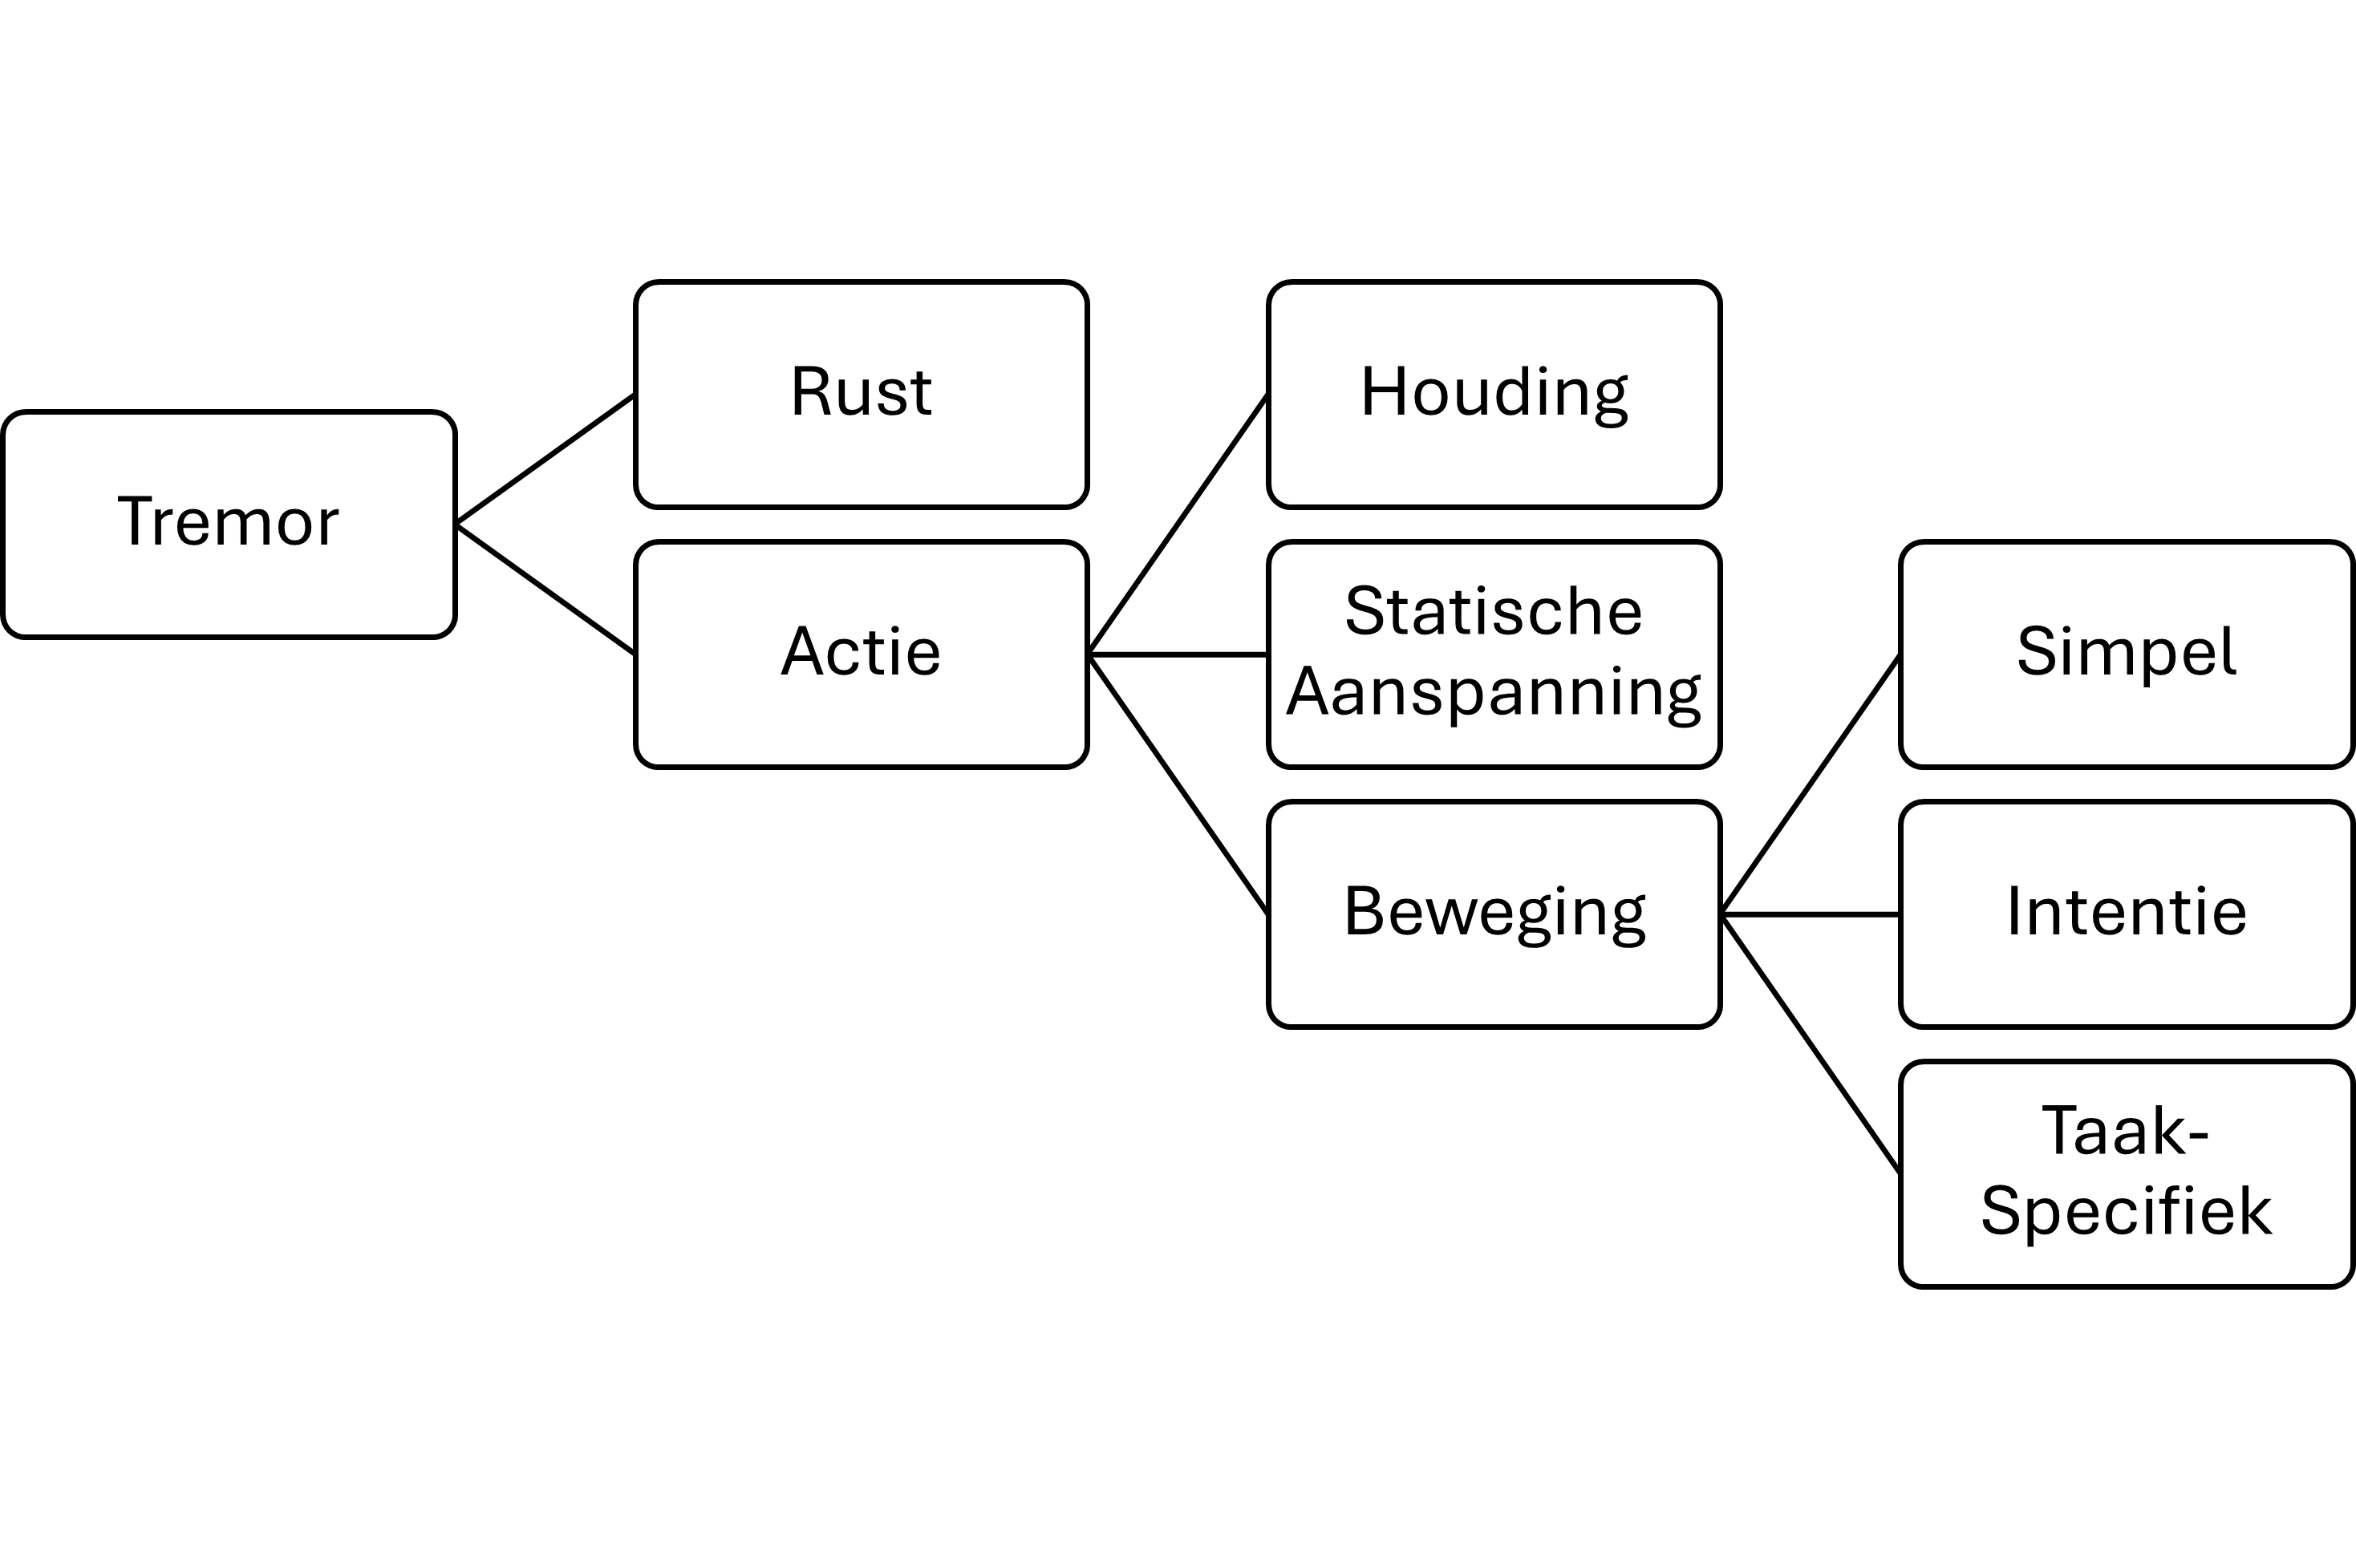
\includegraphics[width=0.4\textwidth]{./graphics/graph-tremor-classification.png}
    \captionof{figure}{Tremor Classification}
    \label{figure:classification}
\end{center}

Een uitgebreide versie van het diagram in Figuur~\ref{figure:classification}
is te vinden in de richtlijnen voor diagnose van het Erasmus MC.
Hierin zijn dezelfde classificaties te zien zoals eerder beschreven, 
met extra informatie die bedoeld is voor, naast de classificatie, de diagnose van een bepaalde tremor\cite{erasmus2022}.
Dit diagram is terug te vinden in bijlage~\ref{appendix:diagnose}.
Gezien dit onderzoek zich richt op de detectie van tremoren, is enkel de classificatie voldoende.

\subsection{Wat is een Essentiële Tremor?}
    \section{Detecteren}
\label{section:detection}

Het doel van dit onderzoek is om te bepalen of tremoren op techniche wijze gedetecteerd kunnen worden.
Dit hoofdstuk beschrijft de huidige methodes om tremoren te detecteren,
waarna er bepaald wordt welke methode het meeste geschikt is voor de rest van het onderzoek.
Dit hoofdstuk geeft antwoord op de vraag: Hoe worden tremoren gedetecteerd?

\subsection{Wat zijn huidige methodes?}

\subsection{Welke methodes zijn geschikt?}
    \section{Prototype}
    \section{Toepassing}
\label{section:application}

Tijdens het schrijven van het laatste hoofdstuk van het onderzoek was het doel om de laatste vraag te beantwoorden:
Hoe kan de data die uit een detectie komt worden gebruikt?
Daarbij wordt er gekeken naar hoe de verkregen kennis in de toekomst kan worden gebruikt om te reageren op metingen.

\subsection{Wat is er geleerd?}

In hoofdstuk~\ref{section:prototyping} is er een prototype gemaakt van een EMG.
Dit is gedaan met vrij simpele en goedkope onderdelen,
waar weinig werk nodig was om gegevens te krijgen uit de elektroden.
Dit laat zien dat het detecteren van tremor goed te doen is.
Het voordeel hierbij is dat frequentie en kracht ideaal zijn om te meten \cite{elsevier2022}.

Als dit mogelijk is met een kleine investering van tijd en geld,
dan zou er veel mogelijk moeten zijn als er in de toekomst gekeken wordt naar mogelijkheden met de GENEActiv \cite{sips2024, activinsights2022}.
Door gegevens te registreren, is het mogelijk om een beeld te krijgen van een tremor in verschillende situaties.
Dit helpt om te bepalen hoe ernstig de tremor is, wanneer een patiënt er het meest last van heeft en hoe de tremor verloopt.

\subsection{Kan dit worden gebruikt?}

In de context van het originele idee,
het toepassen van het concept achter geluidsonderdrukking op tremoren, zou dit bruikbaar moeten zijn.
Geluidsonderdrukking neemt opgenomen geluid, draait het om, en speelt af.
Op deze manier valt het geluid weg \cite{bose2023}.
Geleerd hebbende dat een EMG elektrische spanning in spieren omzet naar geluid,
wetende dat een EMG zowel elektrische spanning kan lezen als geven \cite{knf2022,neuro2009,gohel2020,neurostyle2021},
zou dit moeten kunnen werken. Deze statement is een speculatie en heeft meer onderzoek nodig.

Voor Data Science is het zeker mogelijk om deze data te gebruiken.
In een informeel gesprek met Mischa Beckers, hoofd van het lectoraat Data Science aan de HZ University of Applied Sciences,
is geconcludeerd dat er heel veel informatie te verzamelen is, enkel met een EMG.
Door situaties en opdrachten in een grote dataset correct te labelen, kunnen er vele modellen worden gemaakt.
    \section{Conclusie}
\label{section:conclusion}
    \section{Discussie}
\end{multicols}


{
    \raggedright
    \bibliographystyle{babunsrt}
    \bibliography{tremor-detection}
}

\newpage
\appendix
\section{Diagram voor Diagnose van Tremoren}
\label{appendix:diagnose}

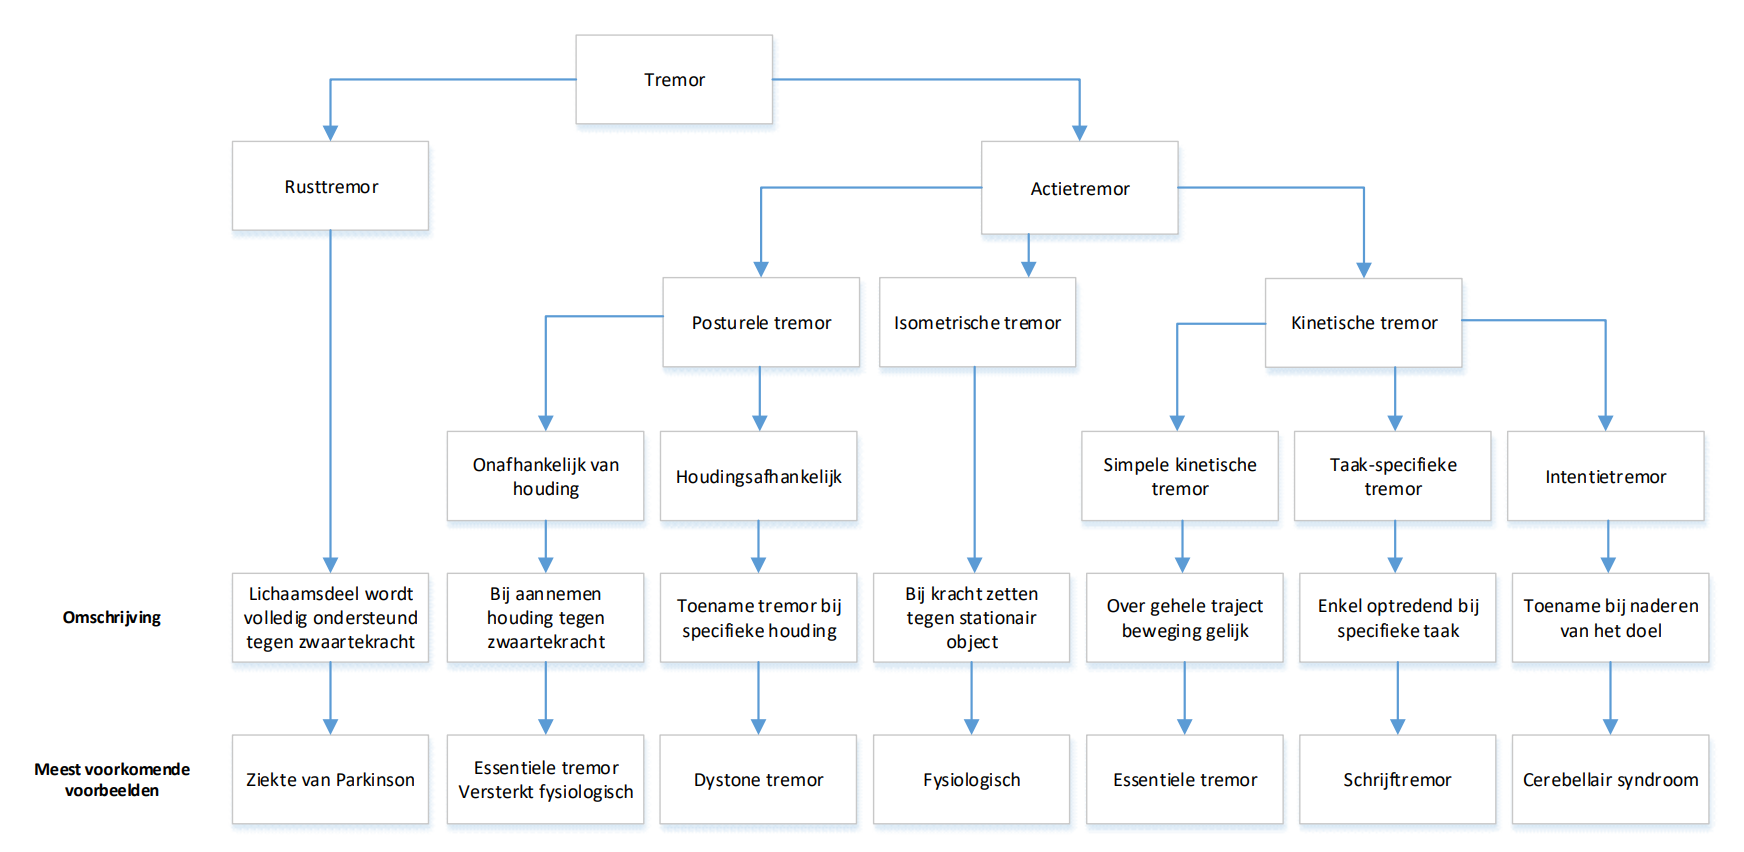
\includegraphics[width=\textwidth]{graphics/graph-tremor-diagnosis.png}

\section{Interview Tremoren en Tremor Registratie}

Tremoren komen het vaakst voor bij Essentiële Tremor en Parkinsons.
Ongeveer 30\% van de gevallen betreft Parkinsons.
Het verschil tussen de twee aandoeningen is dat ET vooral bij actie voorkomt.
Er zijn echter vele variaties van tremoren, welke tremor, is onder andere door de frequentie te meten.

De registratie wordt in het geval van het Admiraal de Ruyter Ziekenhuis gedaan in Vlissingen.
Om van tevoren een inschatting te kunnen maken, kan er gebruik worden gemaakt van apps die trillingen kunnen meten.
Er is wel medicatie beschikbaar voor de aandoening, maar deze zijn niet oorspronkelijk bedoeld voor ET.

Bij Parkinsons valt het resultaat van deze medicatie vaak tegen. Er is dus een vraag naar alternatieven.
Een mogelijke alternatief is DBS (Deep Brain Stimulation). Een ingrijpende, maar effectieve behandeling.
UltraSound is een alternatief dat vooral in Japan wordt gebruikt. Het belooft veel,
maar is nog niet effectief genoeg voor realisatie.

DBS is relatief functioneel en veilig. De behandelingen worden vooral gedaan in Tilburg, Leiden,
Maastricht, Groningen en Amsterdam. Het bestaat 25 jaar en er is experimentele AI voor het lezen en sturen hiervan.

Het registreren van een tremor gebeurd vooral met een EMG (Elektromyogram). Dit brengt spieractiviteit in kaart.
Er zijn polshorloges beschikbaar die dit kunnen meten. 
Deze worden in de praktijk vooral gebruikt voor het meten van stijfheid en overbewegelijkheid.

\end{document}